\documentclass[12pt]{article}
\usepackage{hyperref}
\usepackage{graphicx}
\usepackage{paralist}
\usepackage{amsfonts}
\usepackage{amsmath}
\usepackage{hhline}
\usepackage{booktabs}
\usepackage{multirow}
\usepackage{multicol}
\usepackage{url}

\oddsidemargin 0mm
\evensidemargin 0mm
\textwidth 160mm
\textheight 200mm
\renewcommand\baselinestretch{1.0}

\pagestyle {plain}
\pagenumbering{arabic}

\newcounter{stepnum}

%% Comments

\usepackage{color}

\newif\ifcomments\commentstrue

\ifcomments
\newcommand{\authornote}[3]{\textcolor{#1}{[#3 ---#2]}}
\newcommand{\todo}[1]{\textcolor{red}{[TODO: #1]}}
\else
\newcommand{\authornote}[3]{}
\newcommand{\todo}[1]{}
\fi

\newcommand{\wss}[1]{\authornote{blue}{SS}{#1}}

\title{Assignment 4, Design Specification}
\author{COMPSCI 2ME3}

\begin{document}

\maketitle
This Module Interface Specification (MIS) document contains modules, types and
methods for implementing the game \textit{2048}. At the start of each game, an \textit{4x4} grid with 2 values are given.
The user can move the board either up, down, left, or right. Depending on the move,  the values in the tiles of the board move respectively.
like-numbered values present in the tile when bumped into one-another are merged and added. The main objective of game is to get
the value "2048" by moving the board in different directions and adding like-numbered values. The Game ends when the board is filled with values
except 2048.

\begin{center}
 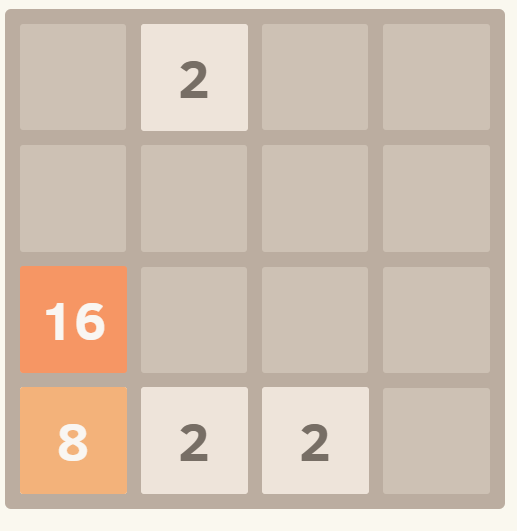
\includegraphics[width=0.55\textwidth]{2048_visual.png}

  The above board visualization is from https://play2048.co/
\end{center}

\newpage

\section{Overview of the design}

This design applies Module View Specification (MVC) design pattern. The MVC components
are \textit{BoardT} (model module), and \textit{Views} (view module). 

\medskip

\begin{flushleft}
The MVC design pattern is specified and implemented in the following way:
\end{flushleft}
 The module \textit{BoardT} stores the state of the game board and the status of the game.\\ A view module \textit{Views} can display
the state of the game board and game using a text-based graphics.\\
\\
For Views, use the getBoard() method to obtain the abstract object.
\bigskip


\subsection*{Likely Changes my design considers:}

\begin{itemize}
  \item Data structure used for storing the game board
  \item The visual representation of the game such. 
\end{itemize}




\newpage

\section* {Board ADT Module}

\subsection*{Template Module inherits EndCondition}

BoardT (with EndCondition)

\subsection* {Uses}

None

\subsection* {Syntax}

\subsubsection* {Exported Types}

None

\subsubsection* {Exported Constant}

Size = 4 \quad // Size of the board 4 x 4

\subsubsection* {Exported Access Programs}

\begin{tabular}{| l | l | l | l |}
\hline
\textbf{Routine name} & \textbf{In} & \textbf{Out} & \textbf{Exceptions}\\
\hline
BoardT & ~ & BoardT & \\
\hline
getBoard & ~ & seq[size] of seq[size] of $\mathbb{N}$  & \\
\hline
getScore & ~ & $\mathbb{N}$ & \\
\hline
Insert\_Random\_Beginning & ~ & ~ & \\
\hline
Insert\_Random & ~ & ~ & \\
\hline
end\_condition\_2048 & ~ & $\mathbb{B}$ & \\
\hline
end\_condition\_filled\_board & ~ & $\mathbb{B}$ & \\
\hline
moveUp & ~ & ~ & \\
\hline
moveDown & ~ & ~ & \\
\hline
moveLeft & ~ & ~ & \\
\hline
moveRight & ~ & ~ & \\
\hline
is\_moveUp & ~ & $\mathbb{B}$ & \\
\hline
is\_moveDown & ~ & $\mathbb{B}$ & \\
\hline
is\_moveLeft & ~ & $\mathbb{B}$ & \\
\hline
is\_moveRight & ~ & $\mathbb{B}$ & \\
\hline
\end{tabular}

\subsection* {Semantics}

\subsubsection* {State Variables}

board: seq[size] of seq[size] of $\mathbb{N}$ \\
score: $\mathbb{N}$

\subsubsection* {State Invariant}

None

\subsubsection* {Assumptions}

\begin{itemize}
  \item The constructor BoardT is called for each object instance before any other access routine 
  is called for that object. 
  \item Assume there is a random function that generates a random value between 0 and 1.
\end{itemize}

\subsubsection* {Access Routine Semantics}

BoardT():
\begin{itemize}
\item transition: \\
      board $:=$ 
      $\langle \begin{array}{c}
      \langle \mbox{0, 0, 0, 0} \rangle\\
      \langle \mbox{0, 0, 0, 0}\rangle\\
      \langle \mbox{0, 0, 0, 0}\rangle\\
      \langle \mbox{0, 0, 0, 0}\rangle\\
      \end{array} \rangle$ \\ 
      score $=$  0
\item output: $out := \mathit{self}$
\item exception: None
\end{itemize}

\noindent getBoard():
\begin{itemize}
\item transition: none
\item output: $out :=$ board
\item exception: None
\end{itemize}

\noindent getScore():
\begin{itemize}
\item transition: none
\item output: $out :=$ score
\item exception: None
\end{itemize}

\noindent Insert\_Random\_Beginning():
\begin{itemize}
\item transition: ( a,b :  $\mathbb{N}$ $\mid$ a, b, c, d $\in$ [0, size - 1] $\implies$ ((board[a][b] = 2 $\lor$ 4) $\land$ (board[c][d] = 2 $\lor$ 4))  )\\

\medskip

\# todo
\item output: $out :=$ none
\item exception: None
\end{itemize}

\noindent Insert\_Random():
\begin{itemize}
\item transition: ( a,b :  $\mathbb{N}$ $\mid$ a, b $\in$ [0, size - 1] $\implies$ (board[a][b] = 2 $\lor$ 4) )\\

\medskip

\# todo
\item output: $out :=$ None
\item exception: None
\end{itemize}

\noindent end\_condition\_2048():
\begin{itemize}
\item transition: None
\item output: $out :=$  ($\forall$ a,b :  $\mathbb{N}$ $\mid$ a, b $\in$ [0, size - 1] : ( board[a][b] = 2048))\\

\medskip

\# todo
\item exception: None
\end{itemize}

\noindent end\_condition\_filled():
\begin{itemize}
\item transition: None
\item output: $out :=$  $\lnot$( $is\_moveUp()$ $\lor$  $is\_moveDown()$ $\lor$ $ is\_moveLeft()$ $\lor$ $ is\_moveRight()$) 

\medskip

\# todo
\item exception: None
\end{itemize}

\noindent moveUp():
\begin{itemize}
\item transition: ($\forall$ a,b :  $\mathbb{N}$ $\mid$ (1 $\le$ a $\textless$ size) $\land$ (0 $\le$ b $\textless$ size)   : ((board[a - 1][b] = 0)  $\Rightarrow$  (board[a - 1][b] =(board[a][b])) 
$\lor$ ((board[a - 1][b] $\neq$ 0) $\land$ (board[a - 1][b] \% 2 = 0) $\land$ ((board[a - 1][b]) = (board[a][b])) $\Rightarrow$ (board[a - 1][b] += board[a][b])))\\

\medskip

\# todo
\item output: $out :=$ None
\item exception: None
\end{itemize}

\noindent moveDown():
\begin{itemize}
\item transition: ($\forall$ a,b :  $\mathbb{N}$ $\mid$ (0 $\le$ a $\textless$ size - 1) $\land$ (0 $\le$ b $\textless$ size)   : ((board[a + 1][b] = 0)  $\Rightarrow$  (board[a + 1][b] =(board[a][b])) 
$\lor$ ((board[a+1][b] $\neq$ 0) $\land$ (board[a+1][b] \% 2 = 0) $\land$ ((board[a + 1][b]) = (board[a][b])) $\Rightarrow$ (board[a + 1][b] += board[a][b])))\\

\medskip

\# todo
\item output: $out :=$ None
\item exception: None
\end{itemize}

\noindent moveLeft():
\begin{itemize}
\item transition: ($\forall$ a,b :  $\mathbb{N}$ $\mid$ (0 $\le$ a $\textless$ size) $\land$ (1 $\le$ b $\textless$ size)   : ((board[a][b - 1] = 0)  $\Rightarrow$  (board[a][b - 1] =(board[a][b])) 
$\lor$ ((board[a][b - 1] $\neq$ 0) $\land$ (board[a][b - 1] \% 2 = 0) $\land$ ((board[a][b - 1]) = (board[a][b])) $\Rightarrow$ (board[a][b - 1] += board[a][b])))\\

\medskip

\# todo
\item output: $out :=$ None
\item exception: None
\end{itemize}

\noindent moveRight():
\begin{itemize}
\item transition: ($\forall$ a,b :  $\mathbb{N}$ $\mid$ (0 $\le$ a $\textless$ size) $\land$ (0 $\le$ b $\textless$ size - 1)   : ((board[a][b + 1] = 0)  $\Rightarrow$  (board[a][b + 1] =(board[a][b])) 
$\lor$ ((board[a][b + 1] $\neq$ 0) $\land$ (board[a][b + 1] \% 2 = 0) $\land$ ((board[a][b + 1]) = (board[a][b])) $\Rightarrow$ (board[a][b + 1] += board[a][b])))\\

\medskip

\# todo
\item output: $out :=$ None
\item exception: None
\end{itemize}

\bigskip

\subsubsection* {Local Functions}

1) is$\_$moveUp : seq[size] of seq[size] of $\mathbb{N}$ $\rightarrow$ $\mathbb{B}$ 

\medskip
\begin{flushleft}
\noindent is$\_$moveUp() $\equiv$  ($\forall$ a,b :  $\mathbb{N}$ $\mid$ (1 $\le$ a $\textless$ size) $\land$ (0 $\le$ b $\textless$ size)   : ((board[a - 1][b] = 0) $\lor$ ((board[a - 1][b]) = (board[a][b])))\\
\end{flushleft}
2) is$\_$moveDown : seq[size] of seq[size] of $\mathbb{N}$ $\rightarrow$ $\mathbb{B}$ 

\medskip
\begin{flushleft}
\noindent is$\_$moveDown() $\equiv$  ($\forall$ a,b :  $\mathbb{N}$ $\mid$ (0 $\le$ a $\textless$ size - 1) $\land$ (0 $\le$ b $\textless$ size)   : ((board[a + 1][b] = 0) $\lor$ ((board[a + 1][b]) = (board[a][b])))\\
\end{flushleft}
3) is$\_$moveLeft : seq[size] of seq[size] of $\mathbb{N}$ $\rightarrow$ $\mathbb{B}$ 

\medskip
\begin{flushleft}
\noindent is$\_$moveLeft() $\equiv$  ($\forall$ a,b :  $\mathbb{N}$ $\mid$ (0 $\le$ a $\textless$ size) $\land$ (1 $\le$ b $\textless$ size)   : ((board[a][b - 1] = 0) $\lor$ ((board[a][b - 1]) = (board[a][b])))\\
\end{flushleft}
4) is$\_$moveRight : seq[size] of seq[size] of $\mathbb{N}$ $\rightarrow$ $\mathbb{B}$ 

\medskip
\begin{flushleft}
\noindent is$\_$moveRight() $\equiv$  ($\forall$ a,b :  $\mathbb{N}$ $\mid$ (0 $\le$ a $\textless$ size) $\land$ (0 $\le$ b $\textless$ size - 1)   : ((board[a][b + 1] = 0) $\lor$ ((board[a][b + 1]) = (board[a][b])))\\
\end{flushleft}


\newpage

\section* {Views Module}

\subsection* {Views Module}

\subsection* {Uses}

BoardT

\subsection* {Syntax}

\subsubsection* {Exported Types}

None

\subsubsection* {Exported Constants}

None

\subsubsection* {Exported Access Programs}

\begin{tabular}{| l | l | l | p{6cm} |}
\hline
\textbf{Routine name} & \textbf{In} & \textbf{Out} & \textbf{Exceptions}\\
\hline
printBoard & BoardT & ~ & \\
\hline
\end{tabular}

\subsection* {Semantics}

\subsection*{Environment Variables}

window: A portion of computer screen is used to print the board and the score.

\subsubsection* {State Variables}

visual: UserInterface

\subsubsection* {State Invariant}

None

\subsubsection* {Access Routine Semantics}

\noindent printBoard($board$):
\begin{itemize}
\item transition: window $:=$ Prints the game board onto the screen. Each 
element is accessed from \textit{BoardT}. The board is displayed as a grid of dimensions 4x4.
\end{itemize}

\newpage


\section*{Critique of Design}

\begin{itemize}
  \item The BoardT module is implemented as an ADT over abstract object. this is mainly because it is more convenient to create a new object each time the game is restarted and for unit testing.
  \item The Views module which represents the View of the MVC design pattern is specefied as an abstract object. This is done so that any unexpected change in the state varibales 
	can be avoided as only one instance of the class is created.
  \item The local functions is\_moveUp(), is\_moveDown(), is\_moveLeft(), is\_moveRight() are not essential we can get the same results from the moveUp(), moveDown(), moveLeft() and 
	moveRight() methods respectively. It was included here to for usability in end\_condition\_filled\_board() method.
  \item The local functions are made public instead of it usually being private. This was done to make testing of local functions with junit possible.
  \item The moveUp(), moveDown(), moveLeft() and moveRight() methods in BoardT module violates the principle of minimality as these methods also update the score as well as the
	state of the board. This was done to make it convenient to calculate the score after each move. 
  \item Test cases generated are used to check the validity and correctness of the the program based on the requirements. Junit was used to impement unit testing due to its friendly and usefull
	framework.
  \item Here the MVC design pattern is used. It is decompsed into model and view and exhibits the principle of seperation of concern as all the two modules have different functionality.
  \item The design used here achieves high cohesion as it related functionalities are grouped with in the same module like the boardT module. low coupling can be observed because each 
	module doesnt depend on each other so a change in my Views model would affect the BoardT module much.
 
  
\end{itemize}

\section*{Answers to Questions:}

Q1: Draw a UML diagram for the modules in A3.\\

\begin{center}
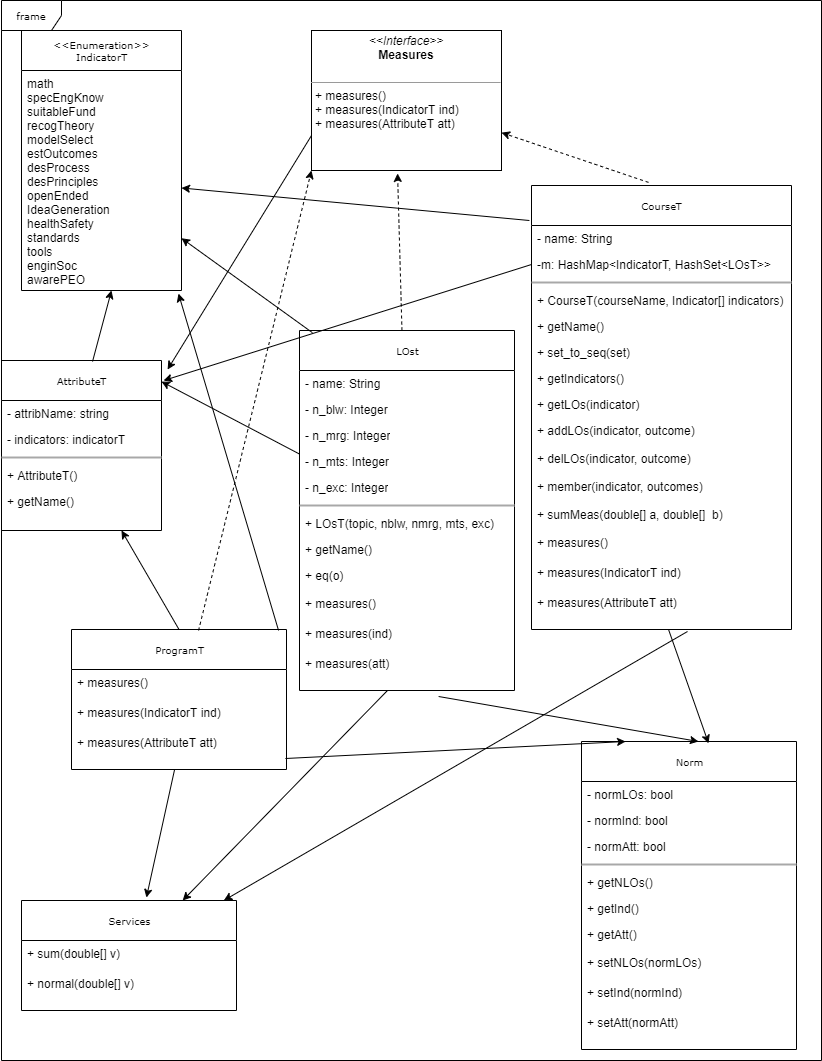
\includegraphics[width=0.9\textwidth]{UML.png}
\end{center}

\medskip
\medskip



\noindent Q2: Draw a control flow graph for the convex hull algorithm.  The graph should
  follow the approach used by the Ghezzi et al.\ textbook.  In particular, the
  code statements should be edges of the graph, not nodes.  Code for the convex
  hull algorithm can be found at:
   https://startupnextdoor.com/computing-convex-hull-in-python/. To match the
  diagrams available from Ghezzi, replace the for loop in the code with a while
  loop.


\begin{center}
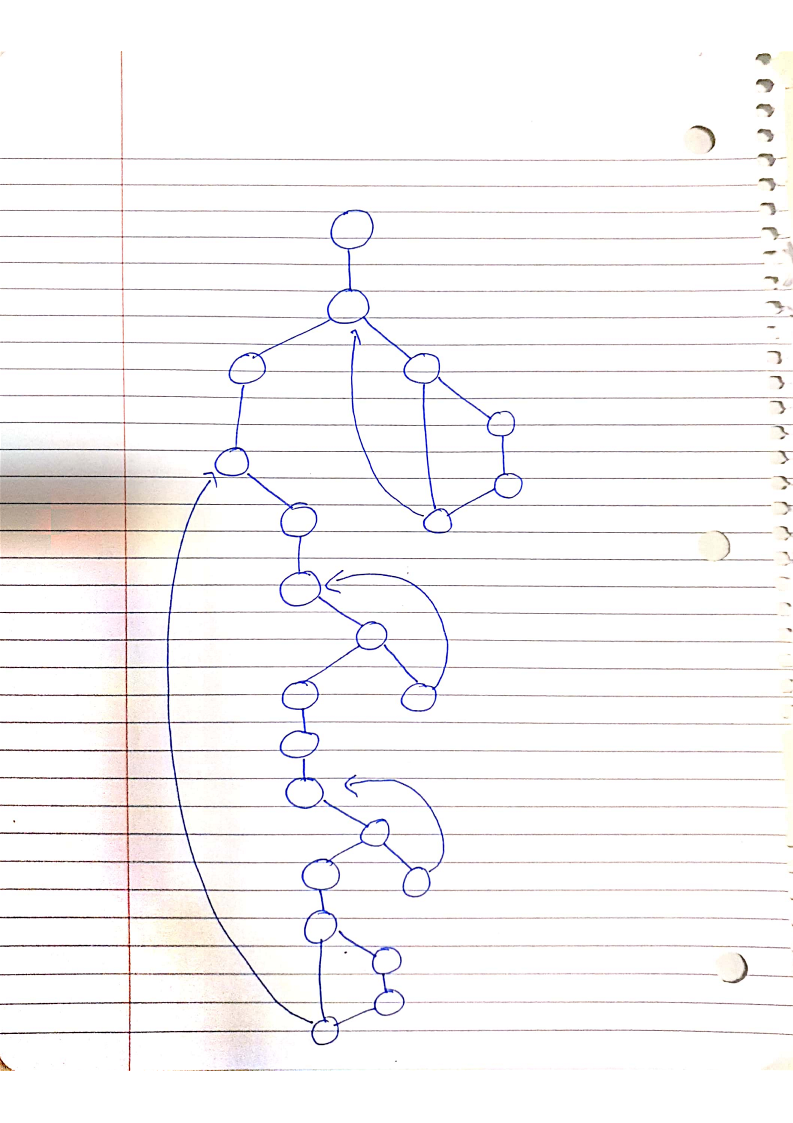
\includegraphics[width=0.9\textwidth]{flow.png}
\end{center}

\subsection* {Citations:}
\begin{itemize}
\item Code reference: https://github.com/gn03249822/Game-2048\%7D\%7B\\https://github.com/gn03249822/Game-2048\%7D
\item MIS: $https://gitlab.cas.mcmaster.ca/smiths/se2aa4_cs2me3/-/tree/master/\\Assignments/PreviousYears/2020$
\end{itemize}

\end {document}